\documentclass{standalone}
\usepackage{tikz}
\usetikzlibrary{patterns}
\usetikzlibrary{positioning}
\usetikzlibrary{patterns, positioning}
\usetikzlibrary{shapes.misc}
\usepackage[outline]{contour}
\contourlength{1.5pt} 
\usepackage[sfdefault]{ClearSans}

\begin{document}
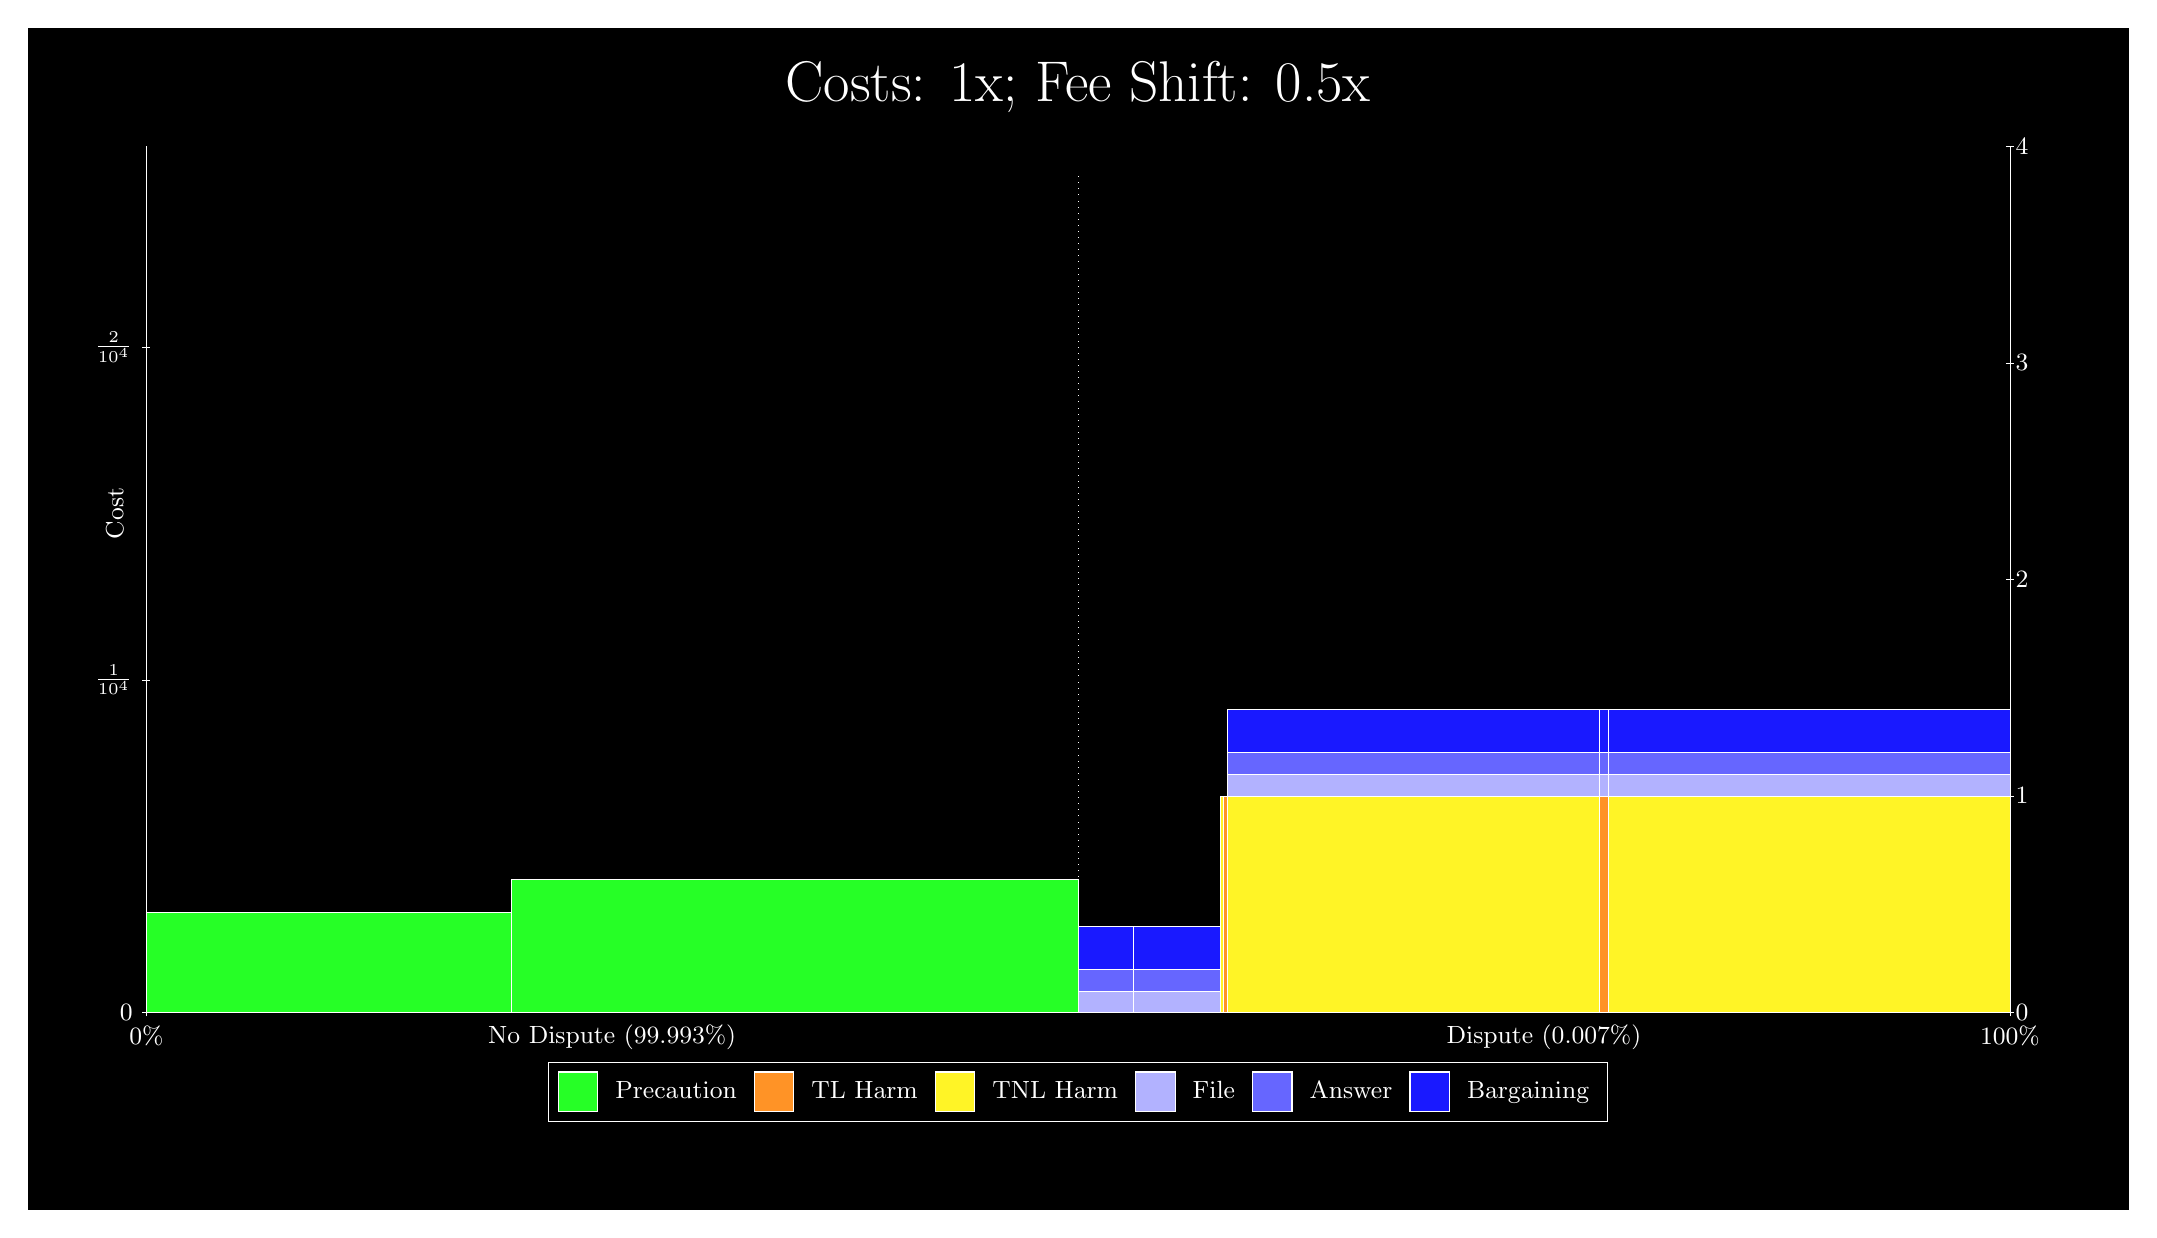
\begin{tikzpicture}
\draw[fill=black] (0,0) rectangle (26.667,15);
\draw[draw=none,text=white] (0,13.5) rectangle (26.667,15) node[midway] {\huge Costs: 1x; Fee Shift: 0.5x };
\draw[fill=green!85,draw=white,very thin] (1.5,2.5) rectangle (6.1372,3.7672);
\draw[fill=green!85,draw=white,very thin] (6.1372,2.5) rectangle (13.333,4.1896);
\draw[fill=green!85,draw=white,very thin] (13.333,2.5) rectangle (14.029,2.5001);
\draw[fill=blue!30,draw=white,very thin] (13.333,2.5001) rectangle (14.029,2.7751);
\draw[fill=blue!60,draw=white,very thin] (13.333,2.7751) rectangle (14.029,3.0501);
\draw[fill=blue!90,draw=white,very thin] (13.333,3.0501) rectangle (14.029,3.6001);
\draw[fill=green!85,draw=white,very thin] (14.029,2.5) rectangle (15.134,2.5001);
\draw[fill=blue!30,draw=white,very thin] (14.029,2.5001) rectangle (15.134,2.7751);
\draw[fill=blue!60,draw=white,very thin] (14.029,2.7751) rectangle (15.134,3.0501);
\draw[fill=blue!90,draw=white,very thin] (14.029,3.0501) rectangle (15.134,3.6001);
\draw[fill=green!85,draw=white,very thin] (15.134,2.5) rectangle (15.182,2.5001);
\draw[fill=yellow!85,draw=white,very thin] (15.134,2.5001) rectangle (15.182,5.2501);
\draw[fill=green!85,draw=white,very thin] (15.182,2.5) rectangle (15.23,2.5001);
\draw[fill=orange!85,draw=white,very thin] (15.182,2.5001) rectangle (15.23,5.2501);
\draw[fill=green!85,draw=white,very thin] (15.23,2.5) rectangle (19.952,2.5001);
\draw[fill=yellow!85,draw=white,very thin] (15.23,2.5001) rectangle (19.952,5.2501);
\draw[fill=blue!30,draw=white,very thin] (15.23,5.2501) rectangle (19.952,5.5251);
\draw[fill=blue!60,draw=white,very thin] (15.23,5.5251) rectangle (19.952,5.8001);
\draw[fill=blue!90,draw=white,very thin] (15.23,5.8001) rectangle (19.952,6.3501);
\draw[fill=green!85,draw=white,very thin] (19.952,2.5) rectangle (20.066,2.5001);
\draw[fill=orange!85,draw=white,very thin] (19.952,2.5001) rectangle (20.066,5.2501);
\draw[fill=blue!30,draw=white,very thin] (19.952,5.2501) rectangle (20.066,5.5251);
\draw[fill=blue!60,draw=white,very thin] (19.952,5.5251) rectangle (20.066,5.8001);
\draw[fill=blue!90,draw=white,very thin] (19.952,5.8001) rectangle (20.066,6.3501);
\draw[fill=green!85,draw=white,very thin] (20.066,2.5) rectangle (25.167,2.5001);
\draw[fill=yellow!85,draw=white,very thin] (20.066,2.5001) rectangle (25.167,5.2501);
\draw[fill=blue!30,draw=white,very thin] (20.066,5.2501) rectangle (25.167,5.5251);
\draw[fill=blue!60,draw=white,very thin] (20.066,5.5251) rectangle (25.167,5.8001);
\draw[fill=blue!90,draw=white,very thin] (20.066,5.8001) rectangle (25.167,6.3501);
\draw[white,very thin] (1.5,2.5) -- (1.5,13.5);
\node[font=\small,rotate=90,text=white, anchor=center] at (1.1, 8.8361) {Cost};
\draw[white,very thin] (1.45,2.5) -- (1.55,2.5);
\node[font=\small,text=white, anchor=east] at (1.45, 2.5) {0};
\draw[white,very thin] (1.45,6.7241) -- (1.55,6.7241);
\node[font=\small,text=white, anchor=east] at (1.45, 6.7241) {$\frac{1}{10^{4}}$};
\draw[white,very thin] (1.45,10.948) -- (1.55,10.948);
\node[font=\small,text=white, anchor=east] at (1.45, 10.948) {$\frac{2}{10^{4}}$};

\draw[white,dotted,very thin] (13.333,2.83) -- (13.333,13.17);
\draw[white,very thin] (25.167,2.5) -- (25.167,13.5);
\draw[white,very thin] (25.117,2.5) -- (25.217,2.5);
\node[font=\small,text=white, anchor=west] at (25.117, 2.5) {0};
\draw[white,very thin] (25.117,5.25) -- (25.217,5.25);
\node[font=\small,text=white, anchor=west] at (25.117, 5.25) {1};
\draw[white,very thin] (25.117,8) -- (25.217,8);
\node[font=\small,text=white, anchor=west] at (25.117, 8) {2};
\draw[white,very thin] (25.117,10.75) -- (25.217,10.75);
\node[font=\small,text=white, anchor=west] at (25.117, 10.75) {3};
\draw[white,very thin] (25.117,13.5) -- (25.217,13.5);
\node[font=\small,text=white, anchor=west] at (25.117, 13.5) {4};

\draw[white,very thin] (1.5,2.5) -- (25.167,2.5);
\draw[white,very thin] (1.5,2.45) -- (1.5,2.55);
\node[font=\small,text=white, anchor=north] at (1.5, 2.45) {0\%};
\draw[white,very thin] (25.167,2.45) -- (25.167,2.55);
\node[font=\small,text=white, anchor=north] at (25.167, 2.45) {100\%};

\node[font=\small,text=white,anchor=south] at (7.4167, 1.9) {No\ Dispute\ (99.993\%)};
\node[font=\small,text=white,anchor=south] at (19.25, 1.9) {Dispute\ (0.007\%)};
\draw (13.3333,2.5) node (B) {};
\begin{scope}[align=center]
\matrix[scale=0.5,draw=white,below=0.5cm of B,nodes={draw},column sep=0.1cm]{
\node[rectangle,draw,minimum width=0.5cm,minimum height=0.5cm,fill=green!85]{}; & \node[draw=none,font=\small,text=white]{Precaution}; &
\node[rectangle,draw,minimum width=0.5cm,minimum height=0.5cm,fill=orange!85]{}; & \node[draw=none,font=\small,text=white]{TL Harm}; &
\node[rectangle,draw,minimum width=0.5cm,minimum height=0.5cm,fill=yellow!85]{}; & \node[draw=none,font=\small,text=white]{TNL Harm}; &
\node[rectangle,draw,minimum width=0.5cm,minimum height=0.5cm,fill=blue!30]{}; & \node[draw=none,font=\small,text=white]{File}; &
\node[rectangle,draw,minimum width=0.5cm,minimum height=0.5cm,fill=blue!60]{}; & \node[draw=none,font=\small,text=white]{Answer}; &
\node[rectangle,draw,minimum width=0.5cm,minimum height=0.5cm,fill=blue!90]{}; & \node[draw=none,font=\small,text=white]{Bargaining}; \\\\
};\end{scope}

\end{tikzpicture}
\end{document}